Zunächst werden der Acrylblock und die Lage der Fehlstellen mittels Schieblehre
bestimmt. Der Block hat eine Höhe von $h=8.07\cm$ und eine Länge von $l=15\cm$.
In Tabelle \ref{tab:oben} sind die Orte der Fehlstellen mit Schieblehre, A-Scan
und B-Scan aufgeführt. Die erste Messung wird so durchgeführt, dass die Bohrung
11 im unteren Teil des Blocks \ref{fig:block} lokalisiert ist. Der A-Scan wurde
mit einer $1\MHz$- und der B-Scan mit einer $2\MHz$-Sonde durchgeführt.
\begin{table}[H]
  \centering
  \begin{tabular}{c|c|cc|cc}
    \toprule
    \multicolumn{1}{c|}{Loch}& \multicolumn{1}{c|}{Schieblehre} & \multicolumn{2}{c|}{A-Scan}
    & \multicolumn{2}{c}{B-Scan} \\
    & $s/\cm$ & $t\ms$ & $s/\cm$ & $t/\ms$ & $s/\cm$ \\
    \midrule
     1  &  1.82 &  17.7 & 2.41 & 15.3 & 2.09 \\
     2  &  1.74 &  15.3 & 2.09 & 14.2 & 1.94 \\
     3  &  6.12 &  46.0 & 6.28 & 45.7 & 6.24 \\
     4  &  5.38 &  40.7 & 5.56 & 40.3 & 5.50 \\
     5  &  4.64 &  35.3 & 4.82 & 35.0 & 4.78 \\
     6  &  3.88 &  29.8 & 4.07 & 29.5 & 4.03 \\
     7  &  3.08 &  24.0 & 3.28 & 23.7 & 3.24 \\
     8  &  2.37 &  18.2 & 2.48 & 17.9 & 2.44 \\
     9  &  1.49 &  12.4 & 1.69 & 12.2 & 1.67 \\
    10  &  0.76 &   6.7 & 0.91 &  6.6 & 0.90 \\
    11  &  5.56 &  42.0 & 5.73 & 41.9 & 5.72 \\
    \bottomrule
  \end{tabular}
  \caption{Lage der Bohrungen von oben.}
  \label{tab:oben}
\end{table}
\noindent Danach wird die Messung erneut durchgeführt, der Block wird jedoch so gedreht,
dass sich Bohrung 11 im oberen Teil des Blocks \ref{fig:block} befindet.
Die Werte für diese Messung sind in Tabelle \ref{tab:unten} zu sehen.
\begin{table}[H]
  \centering
  \begin{tabular}{cc|cc|cc}
    \toprule
    \multicolumn{1}{c}{Loch}& \multicolumn{1}{c|}{Schieblehre} & \multicolumn{2}{c|}{A-Scan}
    & \multicolumn{2}{c}{B-Scan} \\
    & $s/\cm$ & $t/\ms$ & $s/\cm$ & $t/\ms$ & $s/\cm$ \\
    \midrule
     1  &   5.99 &  45.0 & 6.14 & 45.2 & 6.16 \\
     2  &   6.16 &  48.0 & 6.56 & 46.2 & 6.31 \\
     3  &   1.33 &  11.3 & 1.54 & 11.1 & 1.52 \\
     4  &   2.17 &  17.3 & 2.36 & 17.0 & 2.32 \\
     5  &   3.00 &  23.6 & 3.22 & 23.1 & 3.15 \\
     6  &   3.86 &  29.9 & 4.08 & 29.5 & 4.03 \\
     7  &   4.66 &  35.6 & 4.86 & 35.2 & 4.80 \\
     8  &   5.46 &  41.3 & 5.64 & 41.1 & 5.61 \\
     9  &   6.26 &  47.1 & 6.43 & 47.0 & 6.42 \\
    10  &   7.06 &  53.5 & 7.30 & \hrulefill & \hrulefill \\
    11  &   1.55 &  12.7 & 1.73 & 12.4 & 1.69 \\
    \bottomrule
  \end{tabular}
  \caption{Lage der Bohrungen von unten.}
  \label{tab:unten}
\end{table}
\noindent Die Aufnahmebilder des B-Scans sind in Abbildung \ref{fig:bscan} zu sehen.
\begin{figure}[H]
  \centering
  \begin{subfigure}{0.4\textwidth}
    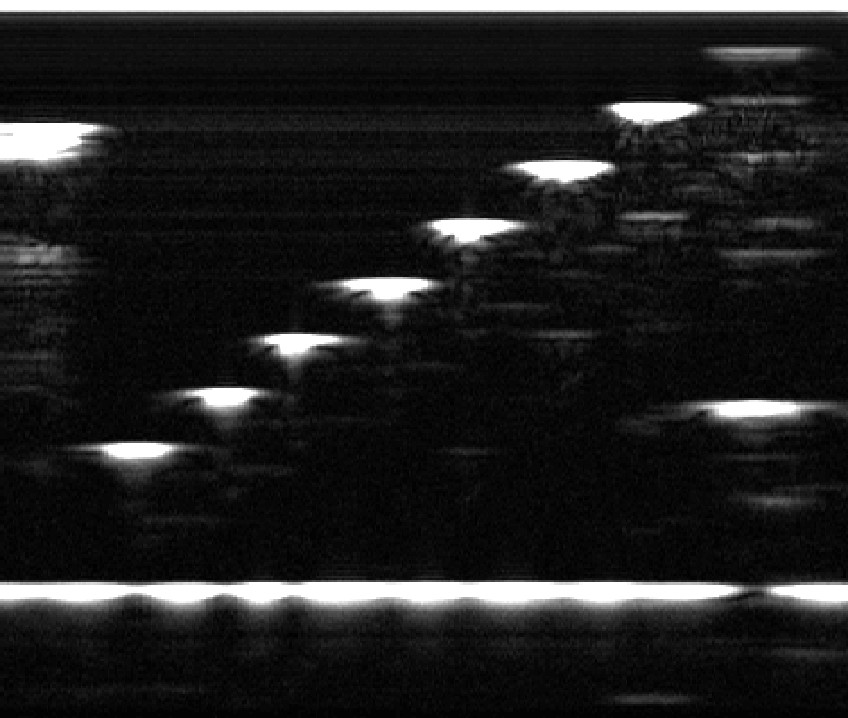
\includegraphics[width=6cm]{bilder/B-ScanUnten.jpg}
    \caption{B-Scan von Oben.}
    \label{sub:oben}
  \end{subfigure}
  \begin{subfigure}{0.4\textwidth}
  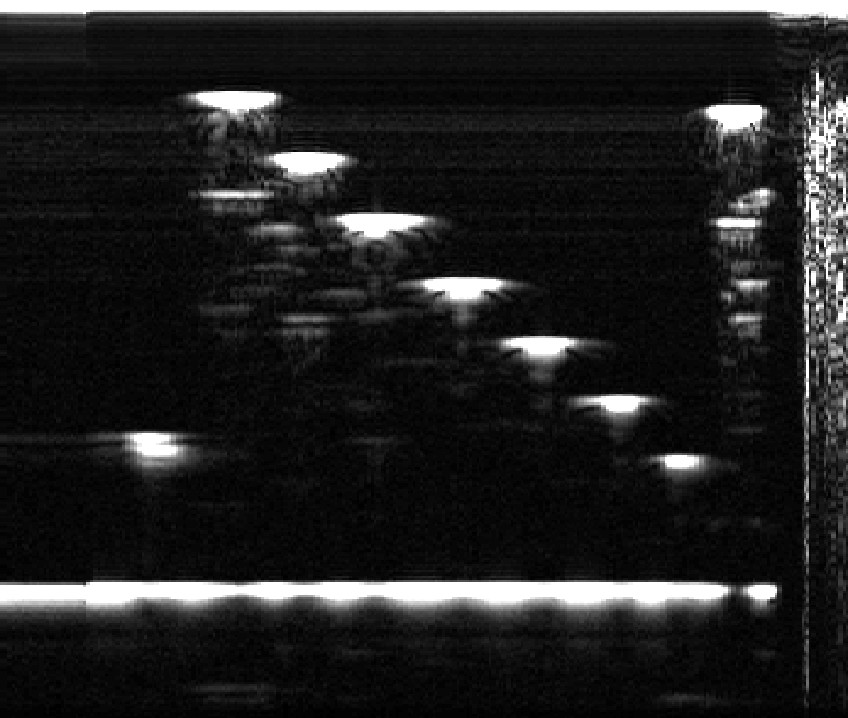
\includegraphics[width=6cm]{bilder/B-ScanOben.jpg}
  \caption{B-Scan von Unten.}
  \label{sub:unten}
\end{subfigure}
\caption{Aufnahmebilder des B-Scans.}
\label{fig:bscan}
\end{figure}
\noindent Hieraus lassen sich die Durchmesser der einzelnen Bohrungen bestimmen, indem
die gemessenen Abstände der Fehlstellen zum Blockrand von der Gesamtblockhöhe
subtrahiert werden. Die einzelenen Durchmesser sind in der untenstehenden
Tabelle \ref{tab:durch} aufgeführt.
\begin{table}[H]
  \centering
  \begin{tabular}{cccc}
    \toprule
    \multicolumn{1}{c}{Loch}&\multicolumn{1}{c}{Schieblehre}&
    \multicolumn{1}{c}{A-Scan}&\multicolumn{1}{c}{B-Scan} \\
    Nummer & $d/\cm$ & $d/\cm$ & $d/\cm$ \\
    \midrule
     1 & 0.26 & -0.37  &  -0.07      \\
     2 & 0.17 & -0.45  &  -0.05      \\
     3 & 0.62 &  0.37  &   0.44      \\
     4 & 0.52 &  0.27  &   0.37      \\
     5 & 0.43 &  0.15  &   0.26      \\
     6 & 0.33 &  0.04  &   0.14      \\
     7 & 0.33 &  0.05  &   0.15      \\
     8 & 0.24 &  0.07  &   0.14      \\
     9 & 0.32 &  0.07  &   0.11      \\
    10 & 0.25 & -0.03  &  \hrulefill \\
    11 & 0.96 &  0.72  &   0.78      \\
    \bottomrule
  \end{tabular}
  \caption{Durchmesser der Fehlstellen.}
  \label{tab:durch}
\end{table}
\noindent Nun wird das Auflösungsverfahren einer $1\MHz$-Sonde mittels A-Scan mit dem
Auflösungsvermögen einer $2\MHz$-Sonde verglichen. Hierfür wird erneut der
Durchmesser für die Löcher 1 und 2 bestimmt.
\begin{table}[H]
  \centering
  \begin{tabular}{ccc}
    \toprule
    \multicolumn{1}{c}{Sonde}&\multicolumn{2}{c}{Durchmesser}\\
    $\nu/\MHz$ & $d_1/\cm$ & $d_2/\cm$ \\
    \midrule
    1  &  -0.37  &  -0.45 \\
    2  &   0.19  &   0.22 \\
    \bottomrule
  \end{tabular}
  \caption{Auflösungsvermögen verschiedener Sonden.}
  \label{tab:auf}
\end{table}
\noindent Als nächstes wird das Herzzeitvolumen des Herzmodells mittels TM-Scan bestimmt.
Das Herzmodell wird im diastolischen Zustand als Kugelsegment, siehe Abb. \ref{fig:kugel},
mit dem Segmentradius $a=2.285\cm$ genähert.
\begin{figure}[H]
  \centering
  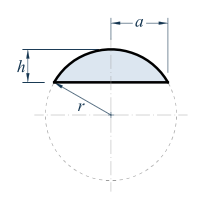
\includegraphics[width=5cm]{bilder/kugel.png}
  \caption{Herzmodell als Kugelsegment \cite{kugel}.}
  \label{fig:kugel}
\end{figure}
\noindent Anhand der aufgenommenen Kurve des TM-Scans, Abb. \ref{fig:tm}, lässt sich sowohl die
Herzfrequenz, als auch das Herzzeitvolumen bestimmen.
\begin{figure}[H]
  \centering
  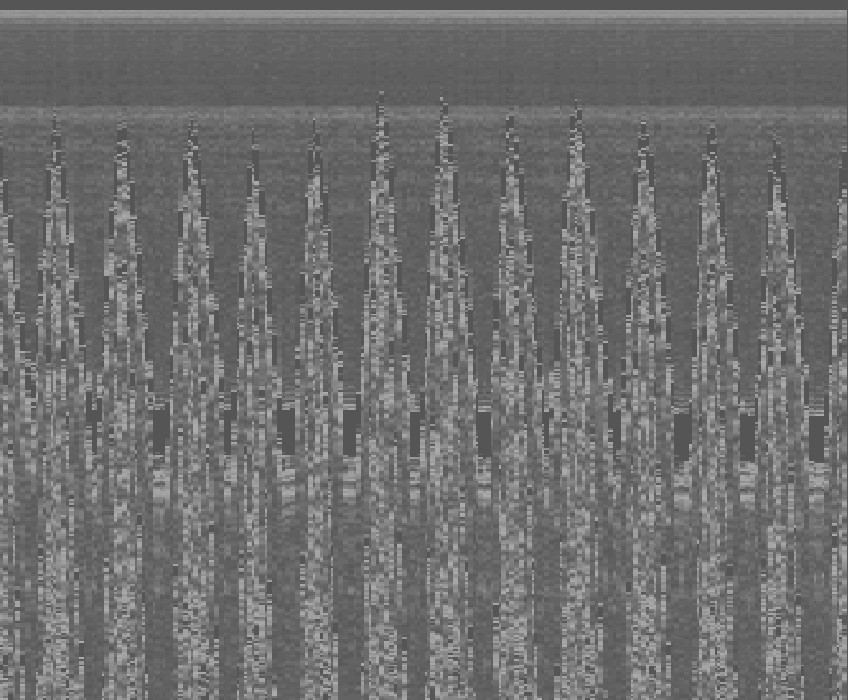
\includegraphics[width=0.6\textwidth]{bilder/TM-ScanHerz2.jpg}
  \caption{Kurve des TM-Scans.}
  \label{fig:tm}
\end{figure}
\noindent Um die Herzfrequenz zu bestimmen werden die Anzahl der Schläge pro Minute
gezählt. In Abbildung \ref{fig:tm} werden 14 Schläge über einen Zeitraum von
$10\sek$ gemessen, woraus sich auf eine Herzfrequenz von $f = 84\,\frac{1}{\si{\minute}}$
schließen lässt.
Um das Herzvolumen zu bestimmen, wird die Laufzeit bei diastolischem, also
relaxierter Membran, von der systolischen, also der kontrahierten, Laufzeit
subtrahiert. Die systolische Laufzeit liegt konstant bei $43.5\ms$.
 Die
Laufzeiten der Diastole sind in Tabelle \ref{tab:dia} einzusehen.
\begin{table}[H]
  \centering
  \begin{tabular}{ccc}
    \toprule
    \multicolumn{1}{c}{Diastole}&\multicolumn{1}{c}{h}&\multicolumn{1}{c}{Herzvolumen}\\
    $t/\ms$ & $h/\cm$ & $V/\ml$ \\
    \midrule
    26.7 & 2.3 & 35.6  \\
    29.2 & 2.0 & 28.8  \\
    28.5 & 2.0 & 30.6  \\
    29.2 & 2.0 & 28.8  \\
    27.9 & 2.1 & 32.2  \\
    29.2 & 2.0 & 28.8  \\
    32.0 & 1.6 & 22.1  \\
    31.5 & 1.6 & 23.2  \\
    29.6 & 1.9 & 27.8  \\
    31.2 & 1.7 & 23.9  \\
    29.0 & 2.0 & 29.3  \\
    28.4 & 2.1 & 30.9  \\
    27.4 & 2.2 & 33.6  \\
    26.3 & 2.3 & 36.7  \\
    \bottomrule
  \end{tabular}
  \caption{Herzvolumen des Herzmodells.}
  \label{tab:dia}
\end{table}
\noindent Die Höhe wird hierbei analog zu dem Durchmesser der Fehlstellen berechnet, jedoch
mit der Schallgeschwindigkeit von Wasser, $c = 1464$ \cite{spektrum}.
Für das Volumen des Kugelsegments gilt
\begin{equation*}
  V=\frac{\pi\cdot h}{6}\lf(3a^2+h^2\rt)\text{\cite{kugel}}.
\end{equation*}
Anhand der Werte lässt sich für das Volumen ein Mittelwert von $\bar V=(14.2\pm1.7)\ml$
berechnen.
Das Herzzeitvolumen wird mit Formel \eqref{eqn:hzv} berechnet. Hierbei wird
$ESV=0$ angenommen.
Das Herzzeitvolumen beträgt somit
\begin{equation*}
  HZV = (1.19 \pm 0.34)\,\si{\litre\per\minute}.
\end{equation*}
Der Fehler wird mit der Gaußschen Fehlerfortpflanzung
\begin{equation*}
  \Delta HZV = \sqrt{f^2\,\cdot\sigma_\su{V}^2}
\end{equation*}
berechnet.
\newpage
